\documentclass[a4paper,12pt]{article}
% Additional Options
\usepackage{booktabs}
\usepackage{enumerate}
\usepackage{multirow}
\usepackage{subfigure}
\usepackage{color}
\usepackage{graphicx}
\usepackage{amsmath}
\usepackage[section]{placeins}
\usepackage{geometry}
\usepackage{float}
\usepackage{xcolor}
\usepackage{listings}
\geometry{left=3.0cm, right=3.0cm, top=2.5cm, bottom=2.5cm}
\usepackage{cite}
\usepackage{setspace}%
\usepackage{indentfirst}
\renewcommand\thesection{\Roman{section}}

\setlength{\parindent}{1.5em}
%\setlength\parskip{.3\baselineskip}

\lstset{ %  
	backgroundcolor=\color{white},   % choose the background color; you must add \usepackage{color} or \usepackage{xcolor}  
	basicstyle=\footnotesize,        % the size of the fonts that are used for the code  
	breakatwhitespace=false,         % sets if automatic breaks should only happen at whitespace  
	breaklines=true,                 % sets automatic line breaking  
	captionpos=bl,                    % sets the caption-position to bottom  
	commentstyle=\color{mygreen},    % comment style  
	deletekeywords={...},            % if you want to delete keywords from the given language  
	escapeinside={\%*}{*)},          % if you want to add LaTeX within your code  
	extendedchars=true,              % lets you use non-ASCII characters; for 8-bits encodings only, does not work with UTF-8  
	frame=single,                    % adds a frame around the code  
	keepspaces=true,                 % keeps spaces in text, useful for keeping indentation of code (possibly needs columns=flexible)  
	keywordstyle=\color{blue},       % keyword style  
	%language=Python,                 % the language of the code  
	morekeywords={*,...},            % if you want to add more keywords to the set  
	numbers=left,                    % where to put the line-numbers; possible values are (none, left, right)  
	numbersep=5pt,                   % how far the line-numbers are from the code  
	numberstyle=\tiny\color{gray}, % the style that is used for the line-numbers  
	rulecolor=\color{black},         % if not set, the frame-color may be changed on line-breaks within not-black text (e.g. comments (green here))  
	showspaces=false,                % show spaces everywhere adding particular underscores; it overrides 'showstringspaces'  
	showstringspaces=false,          % underline spaces within strings only  
	showtabs=false,                  % show tabs within strings adding particular underscores  
	stepnumber=1,                    % the step between two line-numbers. If it's 1, each line will be numbered  
	stringstyle=\color{orange},     % string literal style  
	tabsize=2,                       % sets default tabsize to 2 spaces  
	%title=myPython.py                   % show the filename of files included with \lstinputlisting; also try caption instead of title  
}  


\begin{document}

\begin{spacing}{1.3}%
\vspace*{0.25cm}

\hrulefill

\thispagestyle{empty}

\begin{center}
\begin{large}
\sc{New York University \vspace{0.3em} \\
	Tandon School of Engineering \vspace{0.3em} \\ CS-GY 6643 Computer Vision Spring 2021}
\end{large}

\hrulefill

\vspace*{5cm}

\begin{large}
\sc{{Final Project}}
\end{large}

\vspace{2em}

\begin{large}
\sc{{
\vspace{0.5em}

 Chess Image Recognition Using Traditional Computer Vision Techniques and Neural Networks}}
\end{large}
\end{center}

\vfill

\begin{table}[h!]
\begin{center}
\begin{tabular}{lll}
Name: Tianyi Zhao \hspace*{2em}&
netID: tz1330\\

Name: Zhe Luan \hspace*{2em}&
netID: zl3368\\

 \hspace*{2em} \\
 \\

Date: May 16 2021


\end{tabular}
\end{center}
\end{table}

\newpage


\section{Introduction}

Tencent's Fox Go, a popular go chess game platform which has one of the most powerful go Ai FineArt, has recently released a mobile application which can recognize go chessboard and go pieces. It can output a 2D image of the go-chessboard and help judge the game. Inspired by this application, we want to implement a chess board and chess pieces recognition application. 


\section{Experiment \& Result}

We break this project to two parts, chessboard recognition and chess pieces recognition and positioning. The first part should be straightforward in computer vision. We use traditional CV techniques such as edge detection and Hough transformation.

Different from go pieces, chess pieces recognition is more complicated since there are 6 types of chess pieces of both black and white pieces, so we intend to use some deep learning techniques such as CNN to do this part.


\subsection{Chessboard Coordinates}
We use traditional computer vision techniques to build the chessboard coordinates from an original empty chessboard. First the original chessboard images are transformed to grayscale images and smoothed. Then we use canny edge detection and Hough transform to find the lines. 

The set of lines should be classified to horizontal and vertical sets. We use image K-means clustering with k=2 to classify the lines generated by in the previous steps. Then we can build the chessboard coordinates based by calculating the intersections between each pair of lines in the two sets.

\begin{figure}[H]
	\centering
	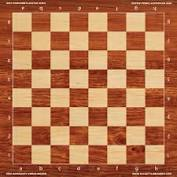
\includegraphics[scale=0.8]{1.jpeg}
	\caption{Original chessboard (1).}
\end{figure}

\begin{figure}[H]
	\centering
	\begin{minipage}[t]{0.45\textwidth}
		\centering
		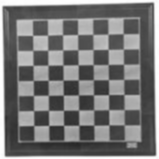
\includegraphics[width=5cm]{2.png}
		\caption{Grayscale and Gaussian blur.}
	\end{minipage}
	\begin{minipage}[t]{0.45\textwidth}
		\centering
		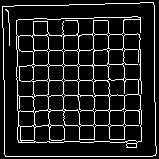
\includegraphics[width=5cm]{3.png}
		\caption{Canny edge detection.}
	\end{minipage}
\end{figure}

\begin{figure}[H]
	\centering
	\begin{minipage}[t]{0.45\textwidth}
		\centering
		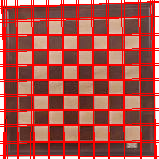
\includegraphics[width=5cm]{4.png}
		\caption{Hough transform.}
	\end{minipage}
	\begin{minipage}[t]{0.45\textwidth}
		\centering
		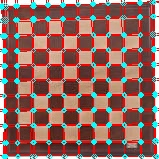
\includegraphics[width=5cm]{5.png}
		\caption{Clustering and intersections.}
	\end{minipage}
\end{figure}

With these methods, we can have good results for different angles of chessboard as the figure shown below.

\begin{figure}[H]
	\centering
	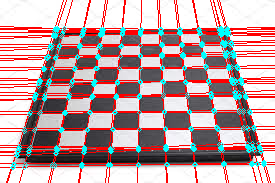
\includegraphics[scale=0.6]{6.png}
	\caption{Chessboard coordinates with different camera angles.}
\end{figure}

When we experimenting on chessboard with pieces, we can generate good coordinates for most cases. However, for each chessboard with different camera angles, we need to manually adjust the parameters of hough transform and line filters.

\begin{figure}[H]
	\centering
	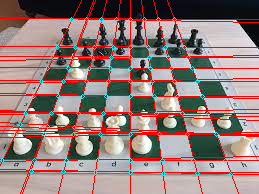
\includegraphics[scale=0.7]{x.png}
	\caption{Chessboard with pieces.}
\end{figure}

\subsection{Chess Piece Classification}

Our dataset consists of 2406 images from twelve types of chess pieces, which are bishops, kings, queens, knights, pawns, rooks in both black and white, and empty cells as the thirteenth piece type. As the example images below show that there are images that have only one chess piece that need to be classified, and also images contain chess pieces. Each type of chess piece has images taken from multiple angles.

\begin{figure}[H]
	\centering
	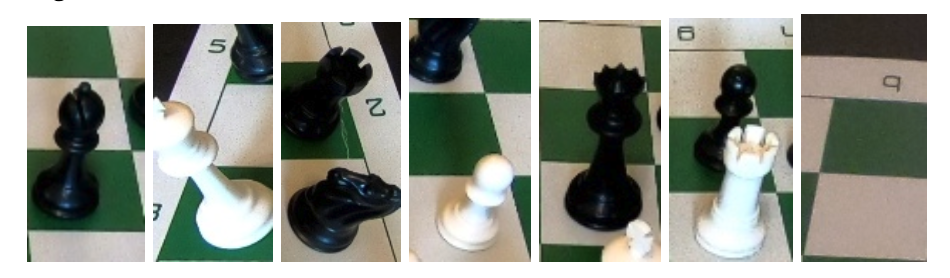
\includegraphics[scale=0.4]{7.png}
	\caption{Examples of images in the dataset.}
\end{figure}

\begin{center}
	\begin{tabular}{|c|c|} \hline
		class &number of images \\ \hline
		black bishop &200 \\  \hline
		black king & 103 \\ \hline
		black knight & 171 \\ \hline
	black pawn & 194 \\ \hline
		black queen& 185 \\ \hline
		black rook& 198 \\ \hline
		empty & 212 \\ \hline
		white bishop & 215 \\ \hline
		white king& 110 \\ \hline
		white knight & 205 \\ \hline
		white pawn & 199 \\ \hline
		white queen& 198 \\ \hline
		white rook& 216 \\ \hline
		total & 2406 \\ \hline
	\end{tabular}
\end{center}

We randomly select 20 images from each class and form a validation dataset of 260 images. (validation dataset with approximately 10% of the whole dataset).  

Convolutional Neural Network has proven to have great performance in image classification tasks, so the team first chose to build a CNN model and train it with our dataset. The CNN model has three convolutional layers, corporate with three max pooling layers to learn the images and extract the useful information and two fully connection layers with Relu activation function to perform predictions of the class of the piece. 

\begin{figure}[H]
	\centering
	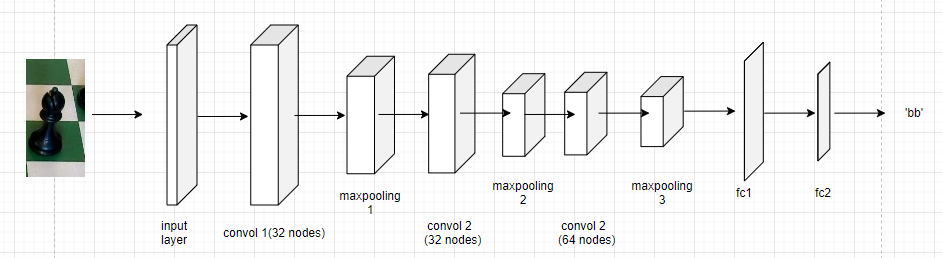
\includegraphics[scale=0.4]{8.png}
	\caption{Structure of CNN model.}
\end{figure}

To build the model, the team chose to use Keras as it provides a high level deep learning framework which is easy to use and set up on google colab where we can access free GPU recourse.  When we feed the data of the image, we rescale the image into size of 224 *224 pixels. Keras data generator module provides the option to alter the data by randomly rotating the image in a given range of angle. We use this feature with setting the range of the rotation to be 0-30 degree, to increase the generalization performance of our model. 

The team also has a concern that given the relatively small size of the accessible dataset, the learning problem might not be learnable for a deep CNN model. So the alternative solution is to utilize the pretrained computer vision models like VGG and Resnet to build a transfer learning model. VGG and Resnet are very deep convolutional networks models with many hidden layers and huge amounts of parameters and they are trained on Imagenet. Transfer learning is a technique that a model trained on a similar dataset as that of the current problem can be used to solve the current problem. Following the standard approach of the transfer learning, the team froze all the parameters in the pretrained models. “Freeze” means that we turn the parameters in the pretrained model to be not learnable so that it would not get updated during the later training. We also remove the fully connected layers, since we are going to train our own fully connected layers to do the predictions. Then we add two fully connected layers on top of the processed pretrained model, then we train the model with our dataset.

\begin{figure}[H]
	\centering
	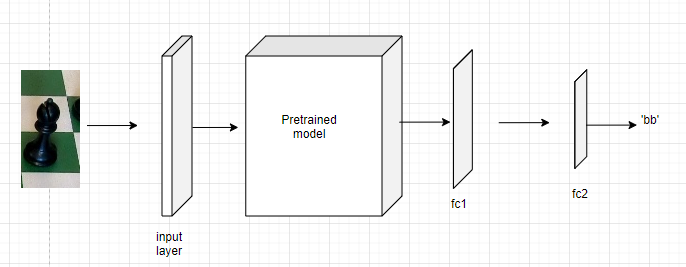
\includegraphics[scale=0.4]{9.png}
	\caption{Structure of the transfer learning model.}
\end{figure}

In the standard approach of transfer learning, there should be one more step of “fine-tuning”, which means we set the parameters inside the pretrained model to be learnable and train the whole model with a very small learning rate. But due to lack of data, we decide not to do this step to prevent overfitting the data.

After the experiment, the performance of the simple CNN model matches the concern of the team. The categorical prediction accuracy on the validation dataset of the model converges around 0.4 in 30 epochs. The model achieved 0.44 as the highest test accuracy. This performance is even worse than random guess which implies that this learning problem is not learnable for the model in the current setting. Following the plan, the team switched to the transfer learning.

We build three models with the same structure of transfer learning model discussed in the previous section by using three different pretrained models: VGG16, VGG19 and Resnet50. The test accuracy of model build with Resnet is unexpectedly bad. The training accuracy and test accuracy converged at the 5th epoch at 0.156 and 0.123. Compared to this, the model uses VGG16 and the model uses VGG 19 get the similar performance in 30 epochs as the figure below shows.

\begin{figure}[H]
	\centering
	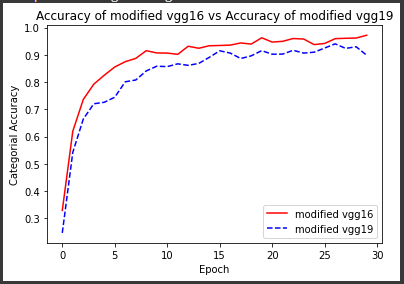
\includegraphics[scale=0.6]{10.png}
	\caption{Test accuracy of the model using VGG16 and the model using VGG19.}
\end{figure}

According to the figure, we can tell that the transfer learning model using VGG16 outperforms the one using VGG19. The best test accuracy of 0.83 is obtained at the 28th epoch, and after that the overfitting occurs.

Therefore, the team chose to use the transfer learning model using VGG16 as our model in chess piece classification. 

\begin{center}
	\begin{tabular}{|c|c|c|c|c|} \hline
		class & Precision & Recall & F1-score & Support \\ \hline
		black bishop & 0.58 & 0.9 & 0.71 &20 \\  \hline
		black king & 0.94 & 0.85 & 0.89 &20 \\  \hline
		black knight & 0.94 & 0.8 & 0.86 &20 \\  \hline
		black pawn & 0.94 & 0.8 & 0.86 &20 \\  \hline
		black queen& 0.93 & 0.7 & 0.8 &20 \\  \hline
		black rook& 0.85 & 0.85 & 0.85 &20 \\  \hline
		empty & 1 & 0.95 & 0.97 &20 \\  \hline
		white bishop & 0.77 & 0.85 & 0.81 &20 \\  \hline
		white king& 1 & 0.9 & 0.75 &20 \\  \hline
		white knight & 0.93 & 0.7 & 0.8 &20 \\  \hline
		white pawn & 0.86 & 0.9 & 0.88 &20 \\  \hline
		white queen& 0.79 & 0.95 & 0.86 &20 \\  \hline
		white rook& 0.62 & 0.9 & 0.73 &20 \\  \hline
	\end{tabular}
\end{center}

The classification report shows that the model has some trouble in classifying black bishops.  This might be due to the fact that the bishops have some sort of similar shape with the pawns with some angles to the focal axis. This explanation is reasonable since the precision for white bishops is also lower than the average precision.

The confusion matrix  of the predictions on the validation data is showing below:

\begin{figure}[H]
	\centering
	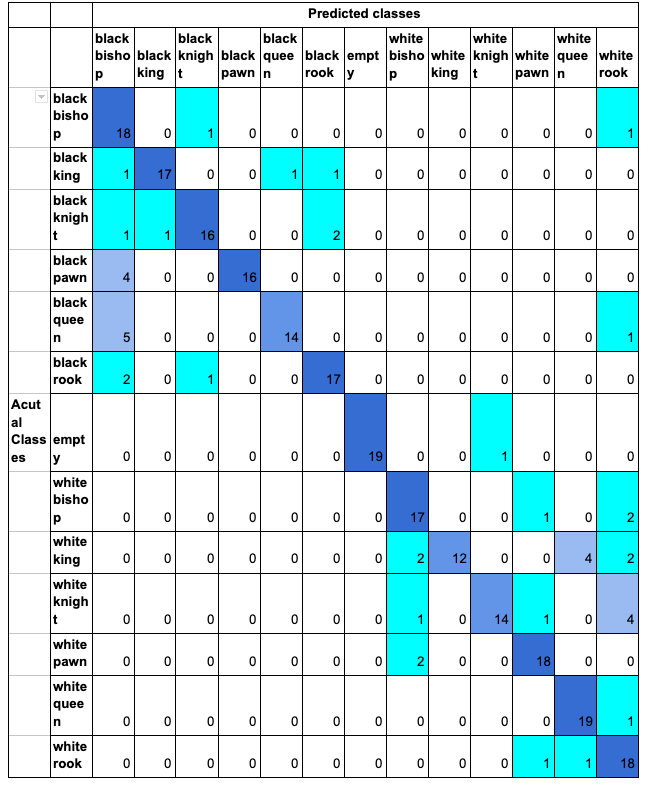
\includegraphics[scale=0.6]{11.png}
\end{figure}


\section{Conclusion}
In this project, we have first used traditional computer vision techniques to recognize chessboard coordinates with different camera angles. With the coordinates we transform the image into many small patches and use the small images to do chess piece classification. By experimenting on different vision networks, we found that VGG16 has a good performance. Then we can combine the coordinates of the chess piece and the classification result to create the visualization of the final chess board.


\section{Further Work}
In chessboard recognition, we need to manually adjust the hough transform parameters for each set of images. A possible way to solve this problem is to scan the parameters and do multiple experiments to figure out if the output number of points is reasonable (between 60 to 100). But if the set of images contains one with no pieces on the chessboard, we can always get the correct coordinates. 

In chess piece classification, there is an obvious problem that, when we divide the transformed chess board into small patches of images containing information of each cell, we are very likely to have several segments of multiple chess pieces inside one small image. And this problem will decrease the accuracy of the classification. One possible work around of this problem is to separate the task of chess piece detection and classification into two subproblems. That is, we first use a machine learning model like YOLO to detect where we have chess pieces on the board, then we map its coordinates to the board by the transformed board coordinates. For this model we need to input a picture of the chess board taken from above of the board. It does not have to have the focal axis perfectly aligned with the normal vector of the plane of the chess board, we can set up an acceptable range of angles. Then we take a picture of the chess board in the same way we have in our current dataset, then we use the coordinates we got from the previous task, and crop each chess piece out from the original image and classify them.

\section{Reference}

\noindent 1. ChessVision: Chess Board and Piece Recognition. Jialin Ding. Stanford University. \\
https://web.stanford.edu/class/cs231a/prev\_projects\_2016/CS\_231A\_Final\_Report.pdf

\vskip\baselineskip
\noindent 2. Chess Piece Recognition Using Oriented Chamfer Matching with a Comparison
to CNN. Youye Xie, Gongguo Tang, William Hoff. Colorado School of Mines, Golden, Colorado USA. \\
https://par.nsf.gov/servlets/purl/10099572

\vskip\baselineskip
\noindent 3. Determining Chess Game State From an Image. Georg Wölflein, Ognjen Arandjelovi´c. \\ https://arxiv.org/pdf/2104.14963.pdf


\end{spacing}
\end{document}